\section{Experimental Details}
\label{app:experimental-details}

In this section, we provide additional details on our experimental setup.

\subsection{Models}
\label{app:experimental-details:models}

\paragraph{\claude{}}

\claude{} has a maximum context of $200$k tokens, but can only process $100$ images at a time. In our setting, a single episode can already consist of up to $100$ images.
As a result, we can, \eg not evaluate in-context learning for \claude{} on Atari.
\claude{} uses approximately $(\mathrm{width~px} \cdot \mathrm{height~px}) / 750$ tokens per image~\citep{anthropic2024vision}.
Finally, note that the monthly token limits for \claude{} are very low compared to the other models (\$$5000$ spend limit per month~\citep{anthropic2024rate}), which is why we can only conduct a somewhat limited evaluation of this model.

\paragraph{\flash{}, \pro{}, and \expflash{}}

The Gemini~$1.5$ models have a maximum context window of $10$ million tokens.
In practice, we restrict ourselves to $1$ million tokens due to the prohibitive cost of evaluating even longer prompts.
The Gemini API considers images to be of fixed size, meaning that they consume a fixed number of tokens (currently $258$), regardless of their file size~\citep{google2024understand}.
\expflash{} supports up to $1$M input tokens and $8$k output tokens~\citep{google2024flash}.

\paragraph{\gpt{}}

The \gpt{} model has a context length of $128$k tokens and can process up to $250$ images per prompt~\citep{openai2024models}.
We use the ``auto'' resolution setting to process the images, which automatically determines whether to use a ``low'' or ``high'' resolution based on the image size~\citep{openai2024vision}.
In the ``low'' resolution mode, the model represents an image with $85$ tokens.
In the ``high'' resolution mode, the model first consumes the low-resolution image (using $85$ tokens) and then creates additional detailed crops of the image using $170$ tokens per $512\mathrm{px} \cdot 512\mathrm{px}$ tile to cover the whole image.

\paragraph{\mini{}, \preview{}, and \oone{}}

\mini{} and \preview{} have a context window of $128$k tokens with up to $65$k output tokens but cannot process images~\citep{openai2024reasoning} so we only evaluate them in the text-based environments (\eg not on Atari).
The \oone{} model has a context window of $200$k tokens and up to $100$k output tokens.


\subsection{Environments}
\label{app:experimental-details:environments}

\paragraph{Visualizing State Representations}

To evaluate \emph{multimodal} in-context imitation learning, we consider multiple state representations for our environments --- which representations exactly depends on the environment.
For example, for chess, we evaluate four different formats: (i) ASCII, (ii) FEN, (iii) PGN, and (iv) RGB images.
We visualize all formats for each environment in \cref{fig:observations-atari,fig:observations-chess,fig:observations-crossword,fig:observations-dm-control,fig:observations-grid-world,fig:observations-tic-tac-toe}.

\begin{figure}[t]
    \begin{minipage}{0.33\textwidth}
        \begin{center}
            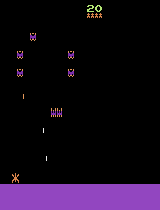
\includegraphics[width=0.5\textwidth]{figures/observations/atari_rgb}
        \end{center}
        \captionof{figure}{An RGB observation for the Phoenix game for Atari 2600.}
        \label{fig:observations-atari}
    \end{minipage}
    \hfill
    \begin{minipage}{0.33\textwidth}
        \begin{center}
            \subfloat[ASCII]{\begin{lstlisting}[basicstyle = \ttfamily, escapeinside={(*}{*)}]
x | o |  
----------
o | x |  
----------
  |   |  
\end{lstlisting}}
            \hfill
            \subfloat[RGB]{
                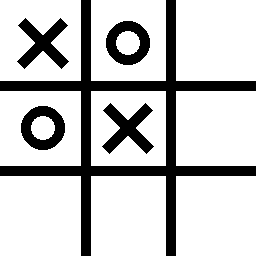
\includegraphics[width=0.35\textwidth,valign=t]{figures/observations/tic_tac_toe_rgb}
            }
        \end{center}
        \caption{Sample observations for each state representation format from our tic-tac-toe environment.}
        \label{fig:observations-tic-tac-toe}
    \end{minipage}
\end{figure}

\paragraph{Atari -- Phoenix}

\begin{figure}
    \begin{center}
        \subfloat[ASCII]{
            \adjustbox{valign=t}{
                \resizebox{0.25\textwidth}{!}{\begin{tabular}{@{}cccccccc@{}}
    r & n & b & q & k & b & n & r \\[1ex]
    p & p & p & p & p & p & p & p \\[1ex]
    . & . & . & . & . & . & . & . \\[1ex]
    . & . & . & . & . & . & . & . \\[1ex]
    . & . & . & . & . & . & . & . \\[1ex]
    . & . & . & . & . & . & . & . \\[1ex]
    P & P & P & P & P & P & P & P \\[1ex]
    R & N & B & Q & K & B & N & R \\[1ex]
\end{tabular}
}
            }
            \label{fig:observation-chess-ascii}
        }
        \hfill
        \subfloat[PGN]{
            \begin{lstlisting}
[Event "World Championship"]
[Site "London"]
[Date "2024.10.29"]
[Round "1"]
[White "Stockfish"]
[Black "Gemini"]
[Result "*"]

1. b3 d5 2. e3 e5 3. c4 *
\end{lstlisting}
            \label{fig:observation-chess-pgn}
        }
        \hfill
        \subfloat[RGB]{
            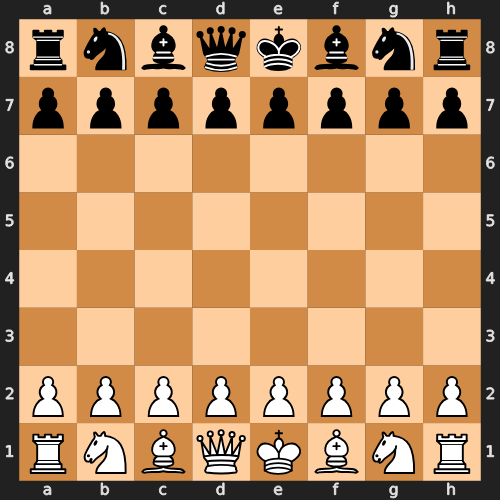
\includegraphics[width=0.25\linewidth,valign=t]{figures/observations/chess_rgb}
            \label{fig:observation-chess-rgb}
        }
    \end{center}
    \par\bigskip
    \begin{center}
        \subfloat[FEN]{           
            \input{figures/observations/chess_fen}
            \label{fig:observation-chess-fen}
        }
    \end{center}
   \caption{
        Sample observations for each state representation format from our chess environment, all of which we generate with the python-chess library~\citep{fiekas2012python}.
        Note that, unlike the ASCII, FEN, and RGB, which show the opening board state, the PGN corresponds to a more advanced position to visualize the move list (which would be empty for the opening board state).
    }
   \label{fig:observations-chess}
\end{figure}

Unlike chess - where a superhuman expert policy (\ie Stockfish) is publicly available, or tic-tac-toe - where the optimal policy can be described with a closed-form algorithm, the best performance on Atari 2600 games is generally obtained by strong reinforcement learning (RL) agents~\citep{mnih2013playing, hessel2021muesli}.
However, rather than training an RL policy from scratch (which can be finicky), we make use of the training data corpus of the Gato project~\citep{reed2022generalist}.
Concretely, Gato trained a Muesli~\citep{hessel2021muesli} agent for $200$M steps and randomly recorded roughly $20$k episodes generated by the agent during training.
As a result, the dataset also contains trajectories from the beginning of training where the agent does not yet perform well, so we only consider the last $2048$ trajectories (\ie the final stages of training).
We further subsample these trajectories by only keeping the $256$ highest-scoring as our expert demonstrations.
Since we only evaluate the first $100$ steps (\ie $400$ frames with an action repeat of $4$), we subsample \wrt the cumulative reward in the first $400$ frames and not \wrt the entire episode.
Overall, we obtain a collection of demonstration episodes with a high average return of $459.9$ in the first $400$ frames. In our experiments we match the Gato setting~\citep{reed2022generalist}, \ie sticky actions and no uncontrolled random initial no-ops. To ensure variability in the evaluation episodes, we manually perform different numbers of no-ops (based on the random seed) at the beginning of every episode before starting the evaluation, which changes the initial state from which the agent has control (since enemies in Phoenix keep moving during this time).



\begin{figure}[t]
    \begin{center}
        \subfloat[Initial crossword]{
            \adjustbox{valign=t}{\begin{lstlisting}[basicstyle = \ttfamily\scriptsize]
+----+----+----+----+----+----+----+
| 01 | ## | ## | 02 |    |    | 03 |
+----+----+----+----+----+----+----+
| 04 |    |    |    | ## | ## |    |
+----+----+----+----+----+----+----+
|    | ## | ## | 05 |    |    |    |
+----+----+----+----+----+----+----+
| 06 | 07 |    | ## | ## | ## |    |
+----+----+----+----+----+----+----+
| ## |    | ## | 08 | 09 |    |    |
+----+----+----+----+----+----+----+
| 10 |    |    | ## |    | ## |    |
+----+----+----+----+----+----+----+
| ## |    | ## | 11 |    |    |    |
+----+----+----+----+----+----+----+

Across:
 2: Go or Go Fish
 4: Texas hold 'em stake
 5: Sierra Club co-founder John
 6: Cueto stat
 8: Eye sore
10: Shorn female
11: Store at a gas station
Down:
 1: Sushi bar libation
 2: It's set in a setting
 3: Sincere, as an apology
 7: Seating sections
 9: Afternoon event in Chelsea
\end{lstlisting}}
            \label{fig:observations-crossword-initial}
        }
        \hspace{64pt}
        \subfloat[Solved crossword]{
            \adjustbox{valign=t}{\begin{lstlisting}[basicstyle = \ttfamily\scriptsize]
+----+----+----+----+----+----+----+
|  S | ## | ## |  G |  A |  M |  E |
+----+----+----+----+----+----+----+
|  A |  N |  T |  E | ## | ## |  A |
+----+----+----+----+----+----+----+
|  K | ## | ## |  M |  U |  I |  R |
+----+----+----+----+----+----+----+
|  E |  R |  A | ## | ## | ## |  N |
+----+----+----+----+----+----+----+
| ## |  O | ## |  S |  T |  Y |  E |
+----+----+----+----+----+----+----+
|  E |  W |  E | ## |  E | ## |  S |
+----+----+----+----+----+----+----+
| ## |  S | ## |  M |  A |  R |  T |
+----+----+----+----+----+----+----+

Across:
 2: Go or Go Fish
 4: Texas hold 'em stake
 5: Sierra Club co-founder John
 6: Cueto stat
 8: Eye sore
10: Shorn female
11: Store at a gas station
Down:
 1: Sushi bar libation
 2: It's set in a setting
 3: Sincere, as an apology
 7: Seating sections
 9: Afternoon event in Chelsea
\end{lstlisting}}
            \label{fig:observations-crossword-solved}
        }
    \end{center}
   \caption{
        Sample observations from our crossword environment.
        \cref{fig:observations-crossword-initial} shows the initial crossword and \cref{fig:observations-crossword-solved} shows the solved crossword after all the words have been placed in their corresponding slots.
        We create the crosswords of size $7\times7$ using the genxword crossword generator~\citep{whitlock2011genxword} and a list of \numprint{55189} clues collected by Matthew Ginsberg (we only use the clues with the lowest difficulty rating; the full list contains \numprint{236615} clues).
   }
   \label{fig:observations-crossword}
\end{figure}

\paragraph{DM Control -- Cheetah Run}

\begin{figure}[t]
    \begin{center}
        \subfloat[Observation]{
            \adjustbox{valign=t}{\begin{lstlisting}[basicstyle = \ttfamily\scriptsize, escapeinside={(*}{*)}]
{
  'position': [-0.09944233298301697, (*$\ldots$*), -0.032929372042417526],
  'velocity': [0.0642457902431488, (*$\ldots$*), 0.1964229941368103],
}
\end{lstlisting}}
        }
        \par\bigskip
        \subfloat[Action]{
            \adjustbox{valign=t}{\begin{lstlisting}[basicstyle = \ttfamily\scriptsize, escapeinside={(*}{*)}]
[-0.8040763139724731, 0.9528138637542725, -1.0, 0.7932683229446411, 1.0, 1.0]
\end{lstlisting}}
        }
    \end{center}
   \caption{
        A sample observation and action from the cheetah run task from the DM Control suite~\citep{tassa2018deepmind}.
        Note that the observation is actually presented to the model on a single line (we use the multi-line representation here for ease of visualization).
        Moreover, we only show the truncated position and velocity vectors (represented by the ellipsis).
        The full position vector contains $8$ elements, and the full velocity vector contains $9$ elements.
        All elements are \texttt{float64} converted to string.
    }
   \label{fig:observations-dm-control}
\end{figure}

There is generally no closed-form or publicly available expert policy for the tasks from the DM Control suite.
Thus, we also leverage the Gato training corpus to generate our expert demonstration episodes for cheetah run.
For this task the Gato project trained a D4PG~\citep{barth2018distributed} agent, and, like for Atari, we only consider the last $10$k episodes (since those correspond to the later stages of training and thus better performance). 
Ideally we would want to subsample the highest-scoring trajectories as expert demonstrations, but, unfortunately, the underlying MuJoCo~\citep{todorov2012mujoco} physics have changed since the time of the Gato data collection, which means that the rewards in the dataset no longer match the observation-actions pairs in our DM Control environment (\ie replaying the actions from the same initial state does not yield the same return).
Thus, we first replay the actions for every trajectory in our collection (setting the initial state based on the first observation) and use the new returns to subsample the $1000$ highest-scoring trajectories (again only considering the cumulative reward in the first $100$ steps).
Overall, we obtain a collection of demonstration episodes with a high average return of $37.4$ in the first $100$ steps.

\begin{figure}[t]
    \begin{center}
        \subfloat[ASCII]{\begin{lstlisting}[basicstyle = \ttfamily\tiny, escapeinside={(*}{*)}]
-------------------------------------------------------------------------------------------------------------
|  wall  |  wall  |  wall  |  wall  |  wall  |  wall  |  wall  |  wall  |  wall  |  wall  |  wall  |  wall  |
-------------------------------------------------------------------------------------------------------------
|  wall  |  tile  |  tile  |  tile  |  tile  |  tile  |  tile  |  tile  |  tile  |  tile  |  tile  |  wall  |
-------------------------------------------------------------------------------------------------------------
|  wall  |  tile  |  tile  |  tile  |  tile  |  tile  |  tile  | player |  tile  |  tile  |  tile  |  wall  |
-------------------------------------------------------------------------------------------------------------
|  wall  |  tile  |  tile  |  tile  |  tile  |  tile  |  tile  |  tile  |  tile  |  tile  |  tile  |  wall  |
-------------------------------------------------------------------------------------------------------------
|  wall  |  tile  |  tile  |  tile  |  tile  |  tile  |  tile  |  tile  |  tile  |  tile  |  tile  |  wall  |
-------------------------------------------------------------------------------------------------------------
|  wall  |  tile  |  tile  |  tile  |  tile  |  tile  |  tile  |  tile  |  tile  |  tile  |  tile  |  wall  |
-------------------------------------------------------------------------------------------------------------
|  wall  |  tile  | target |  tile  |  tile  |  tile  |  tile  |  tile  |  tile  |  tile  |  tile  |  wall  |
-------------------------------------------------------------------------------------------------------------
|  wall  |  tile  |  tile  |  tile  |  tile  |  tile  |  tile  |  tile  |  tile  |  tile  |  tile  |  wall  |
-------------------------------------------------------------------------------------------------------------
|  wall  |  tile  |  tile  |  tile  |  tile  |  tile  |  tile  |  tile  |  tile  |  tile  |  tile  |  wall  |
-------------------------------------------------------------------------------------------------------------
|  wall  |  tile  |  tile  |  tile  |  tile  |  tile  |  tile  |  tile  |  tile  |  tile  |  tile  |  wall  |
-------------------------------------------------------------------------------------------------------------
|  wall  |  tile  |  tile  |  tile  |  tile  |  tile  |  tile  |  tile  |  tile  |  tile  |  tile  |  wall  |
-------------------------------------------------------------------------------------------------------------
|  wall  |  wall  |  wall  |  wall  |  wall  |  wall  |  wall  |  wall  |  wall  |  wall  |  wall  |  wall  |
-------------------------------------------------------------------------------------------------------------
\end{lstlisting}}
        \par\bigskip
        \subfloat[Coordinates]{\begin{lstlisting}[basicstyle = \ttfamily\scriptsize, escapeinside={(*}{*)}]
{'player': [2, 7], 'target': [6, 2]}
\end{lstlisting}}
        \hfill
        \subfloat[RGB]{
            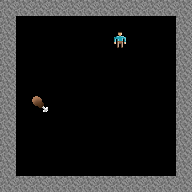
\includegraphics[width=0.25\linewidth,valign=t]{figures/observations/grid_world_rgb}
            \label{fig:observations-grid-world-rgb}
        }
    \end{center}
   \caption{
        Sample observations from our grid world environment for all three state representation formats.
        For the RGB observations (\cref{fig:observations-grid-world-rgb}), we use the sprites from Crafter~\citep{hafner2022benchmarking} for the walls, the player, and the target (the floor is a black square).
    }
   \label{fig:observations-grid-world}
\end{figure}


\subsection{Prompts}
\label{app:experimental-details:prompts}

The frozen part and the dynamic part of the evaluation prompt are illustrated in \cref{code:frozen-prompt} and \cref{code:dynamic-prompt}, respectively.

\begin{listing}
    \caption{
        The frozen part of the evaluation prompt, which contains the expert demonstration episodes and stays constant throughout an evaluation episode.
        In this example, we have 8 demonstration episodes with 10 steps each and RGB observations.
        Before feeding the prompt to the model, we replace the observation and action placeholders with the actual observations (\ie images in this case) and action strings.
    }
    \label{code:frozen-prompt}
   \begin{minted}[mathescape,
               fontsize=\footnotesize,
               linenos,
               numbersep=5pt,
               gobble=7,
               frame=lines,
               framesep=2mm]{python}
        demonstration_prompt = '''
        You are a powerful reinforcement learning agent. You can effectively identify a policy
        exposed by demonstrations and reproduce it in a new situation.
        
        Here are a number of demonstrations:
        
        Observation: <IMG_0_0> Action: <AC_0_0>
        Observation: <IMG_0_1> Action: <AC_0_1>
        ...
        Observation: <IMG_0_9> Action: <AC_0_9>
        
        Observation: <IMG_1_0> Action: <AC_1_0>
        Observation: <IMG_1_1> Action: <AC_1_1>
        ...
        Observation: <IMG_1_9> Action: <AC_1_9>
        
        ...
        
        Observation: <IMG_7_0> Action: <AC_7_0>
        Observation: <IMG_7_1> Action: <AC_7_1>
        ...
        Observation: <IMG_7_9> Action: <AC_7_9>
        '''
    \end{minted}
\end{listing}

\begin{listing}
    \caption{
        The dynamic part of the evaluation prompt containing the evaluation trajectory.
        While stepping through an environment, we append this prompt to the one in \cref{code:frozen-prompt} in every evaluation step (\eg for the 3rd step here), again replacing the observation and action placeholders with the actual observations and actions.
        This example also shows the legal moves (lines $8$ to $10$) and uses chain-of-thought prompting (lines $12$ to $17$, \citet{wei2022chain}), both of which may be omitted depending on our ablations in \cref{app:additional-results:ablations} (which can vary for each model-task combination).
    }
    \label{code:dynamic-prompt}
    \begin{minted}[mathescape,
               fontsize=\footnotesize,
               linenos,
               numbersep=5pt,
               gobble=7,
               frame=lines,
               framesep=2mm]{python}
        evaluation_prompt = '''
        This is the current situation:
        
        Observation: <IMG_8_0> Action: <AC_8_0>
        Observation: <IMG_8_1> Action: <AC_8_1>
        Observation: <IMG_8_2>
        
        In this situation, this is the list of all the moves that are legal:
        
        no action, jump left, left
        
        Given the demonstrations and the current situation, you should infer the next logical
        action. Check that the chosen action is in the set of legal moves. Think step by step
        and very briefly explain your reasoning for choosing this  action. You must answer with
        the reasoning followed by the action in the following format:
        Reasoning: ...
        Action: ...
        '''
    \end{minted}
\end{listing}

